\begin{figure}[p]
\centering
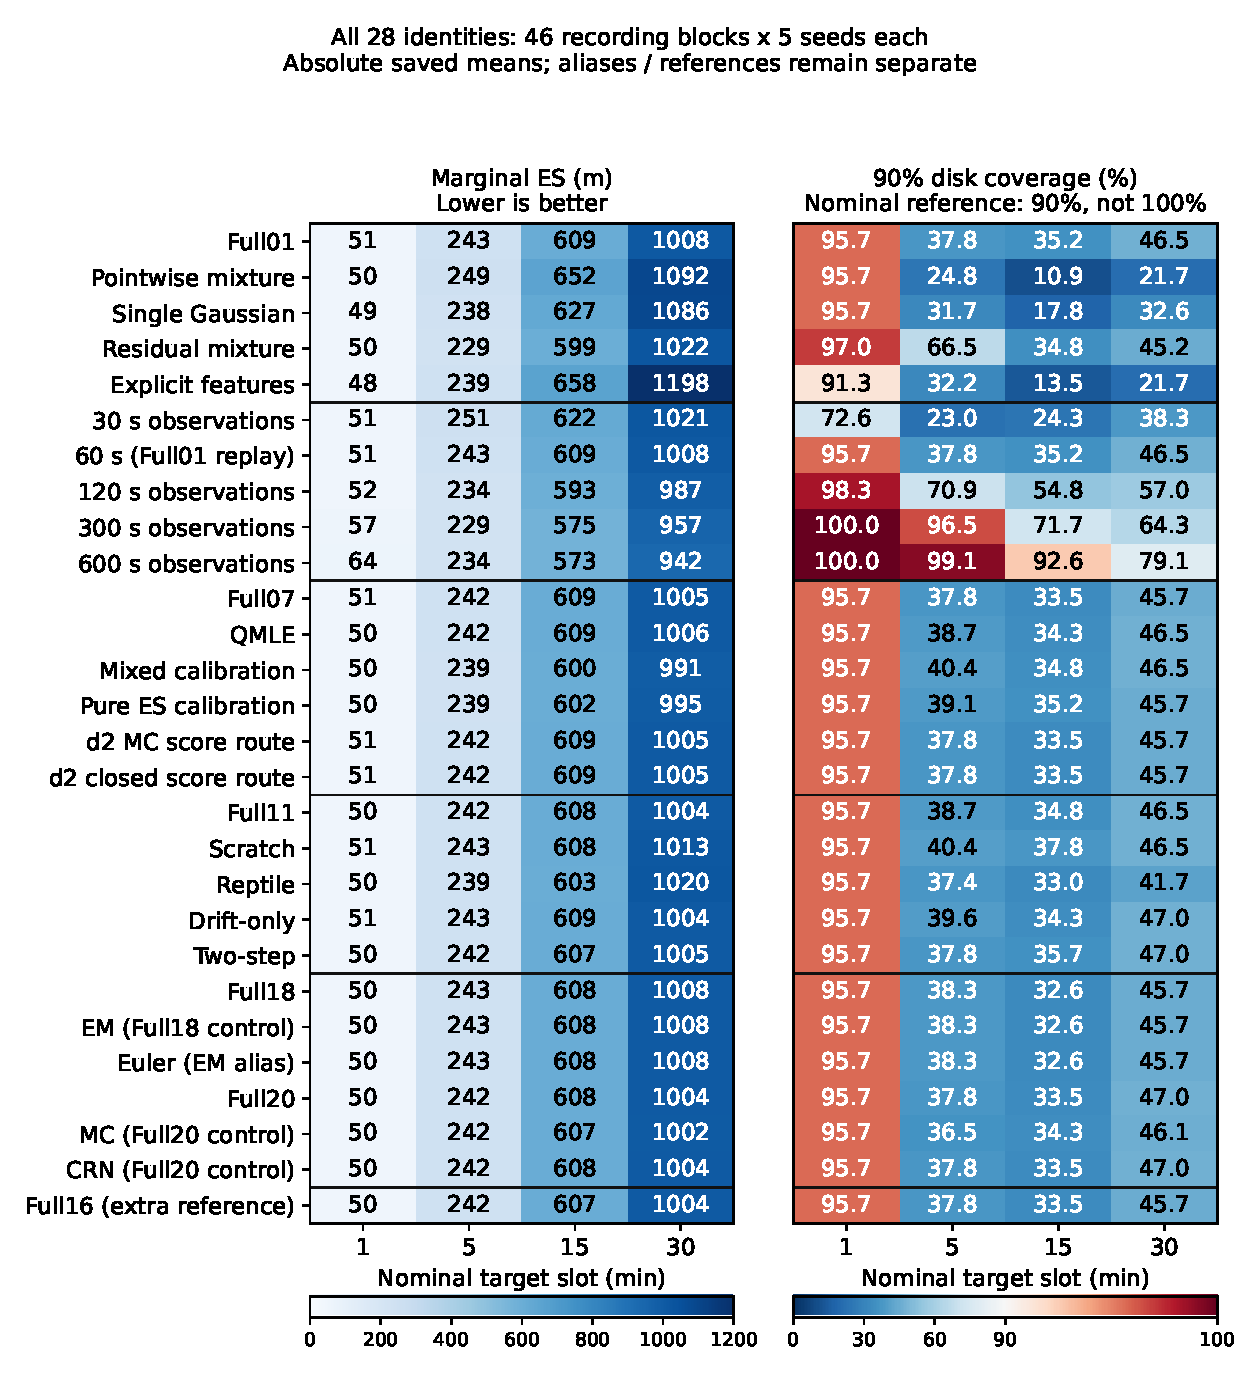
\includegraphics[height=.79\textheight,width=\linewidth,keepaspectratio]{../figures/revision46-corrections-v1/method-horizon-overview.pdf}
\caption{All 28 primary saved configurations at four nominal target slots; no intermediate-time prediction is added. Left: marginal ES (m), lower is better. Right: empirical nominal 90\% disk coverage (\%); 90\% is the calibration reference, not 100\%, and region sizes are not shown. Each cell averages the same 46 blocks and five seeds. ES is rounded to whole metres and coverage to one decimal for overview only; full-precision values and all roles remain in the saved projection and Table~\ref{tab:all-method-horizons}. Row order follows the declared families, not performance. Aliases and distinct Full controls are not pooled; similar rounded cells do not establish equivalence. Descriptive, not new per-horizon tests or final qualification.}
\label{fig:all-method-horizons}
\end{figure}
